
\documentclass[12pt,a4paper]{article}

\usepackage[a4paper,margin=1in]{geometry}
\usepackage{graphicx}
\usepackage{booktabs}
\usepackage{amsmath,amssymb}
\usepackage{float}
\usepackage{hyperref}
\usepackage{xcolor}
\usepackage{listings}
\usepackage{enumitem}
\usepackage{fancyhdr}
\usepackage{longtable}

\hypersetup{colorlinks=true,linkcolor=blue,urlcolor=blue}

\pagestyle{fancy}
\fancyhf{}
\lhead{ICS1512}
\rhead{Machine Learning Algorithms Laboratory}
\cfoot{\thepage}

\lstset{
language=Python,
basicstyle=\ttfamily\small,
numbers=left,
frame=single,
breaklines=true,
showstringspaces=false
}

\begin{document}

\begin{tabular}{|p{4cm}|p{11cm}|}
\hline
Experiment No. & 1 \\ \hline
Experiment Title & Working with Python packages - Numpy, Scipy, Scikit-Learn, Matplotlib\footnotemark \\ \hline
Student Name & Sanjay S \\ \hline
Register Number & 3122247001056 \\ \hline
Faculty & Dr. Poreddy Ajay Kumar Reddy \\ \hline
Submission Date & 03/08/2026 \\ \hline
\end{tabular}
\footnotetext{\textbf{GitHub Repository: }\url{https://github.com/sanjay-6727/Introdution-to-Machine-Learning-}}

\section{Objective}
Get comfortable with Numpy, Pandas, Scipy, Scikit-learn and Matplotlib, and practice the standard ML
workflow (load, explore, clean, split, evaluate) on five different datasets so I could actually see the
right category of problem before jumping into any modeling.

\section{Problem Statement}
Given five public datasets that each cover a different kind of learning problem, load each one, figure
out whether it calls for classification or regression, clean it up, split it, and train a small baseline
model just to prove the pipeline actually runs end to end.

\section{Dataset Description}
\begin{longtable}{|p{3.3cm}|p{2.6cm}|p{1.6cm}|p{1.8cm}|p{1.6cm}|p{2cm}|}
\hline
\textbf{Dataset} & \textbf{Source} & \textbf{Samples} & \textbf{Features} & \textbf{Classes} & \textbf{Missing} \\ \hline
Iris & scikit-learn built in & 150 & 4 & 3 & none \\ \hline
Loan Amount Prediction & Kaggle, phileinsophos\slash predict-loan-amount-data & 29660 & 20 & regression target & 24327 cells across several columns \\ \hline
Predicting Diabetes & Kaggle, uciml\slash pima-indians-diabetes-database & 768 & 8 & 2 & none recorded, though several medical fields use 0 as a placeholder \\ \hline
Email Spam (Spambase) & Kaggle, somesh24\slash spambase & 4601 & 57 & 2 & none \\ \hline
Handwritten Digits & scikit-learn built in (digits, used as an MNIST style stand in) & 1797 & 64 & 10 & none \\ \hline
\end{longtable}

Each one got split roughly 60/20/20 into train, validation and test, stratified wherever the task was
classification.

\section{Exploratory Data Analysis}
\begin{itemize}
\item Dataset overview and statistical summary: histogram, box plot and violin panels per dataset.
\item Missing value analysis: loan data has real gaps, the other four are basically complete.
\item Class distribution and correlation: pair plots and correlation heatmaps, one set per dataset.
\end{itemize}

\begin{figure}[H]
\centering
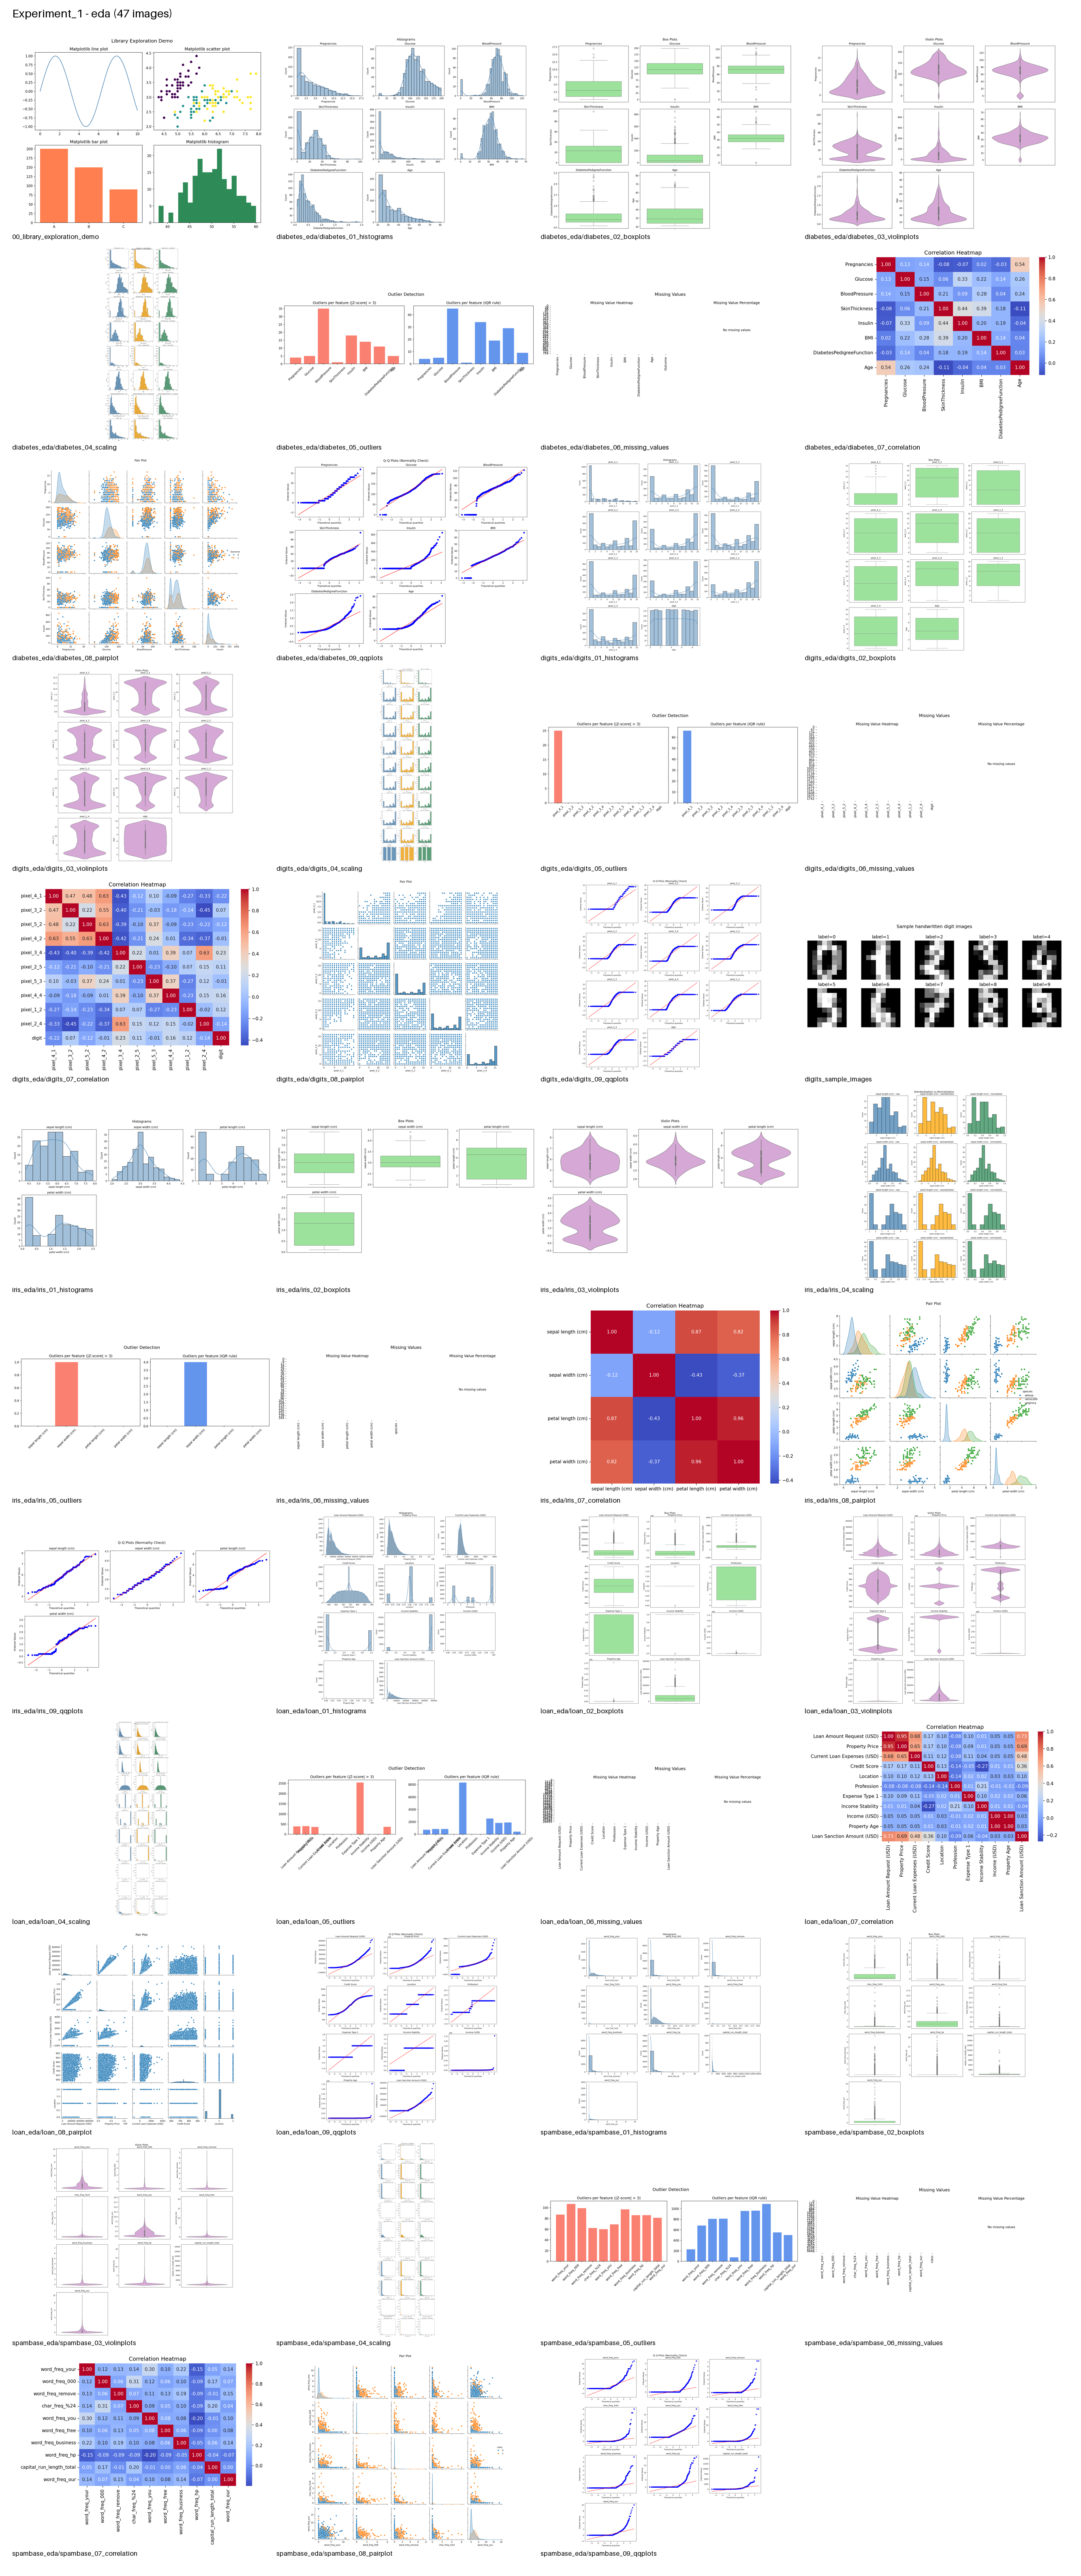
\includegraphics[width=0.95\linewidth]{outputs/Experiment_1_eda_combined.png}
\caption{Combined EDA sheet for all five datasets: histograms, box plots, violin plots, scaling
comparison, outliers, missing values, correlation, pair plots and Q-Q plots, plus a sample of digit
images.}
\end{figure}

\textbf{Inference:}

First thing that jumped out on Iris was petal length and petal width being almost perfectly correlated,
around 0.96, which already hints one of them is doing most of the work in separating species. The loan
missing-value heatmap makes Type of Employment and Property Age look like the worst offenders by a wide
margin. Spambase's word frequency histograms are all heavily right skewed with a big spike at zero, not
surprising really, since most emails just do not contain most of the tracked words at all. The digit
samples were a nice sanity check too, you can actually see how blocky an 8x8 pixel image is once you look
at it directly instead of just trusting the shape numbers. On the outlier side, Diabetes and Loan Amount
both carry noticeably more of them than Iris, which tracks with Iris being a small, curated teaching
dataset rather than something scraped from the real world.

\section{Data Preprocessing}
\begin{itemize}
\item Missing values: loan's numeric columns filled with the median, categorical columns with the mode.
\item Encoding: loan's categorical columns got label encoded, everything else was already numeric.
\item Scaling: every feature matrix was standardized with StandardScaler before modeling.
\item Split: 60/20/20 train/validation/test, stratified for the classification tasks.
\item Loan's identifier columns (Customer ID, Name, Property ID) were dropped before modeling since
they obviously carry no signal.
\end{itemize}

\begin{lstlisting}[caption={Same pattern reused across all five datasets: split, scale, fit, evaluate}]
X_train, X_test, y_train, y_test = train_test_split(
    X, y, test_size=0.2, random_state=42, stratify=y)

scaler = StandardScaler().fit(X_train)
X_train_s = scaler.transform(X_train)
X_test_s = scaler.transform(X_test)

model = LogisticRegression(max_iter=1000).fit(X_train_s, y_train)
pred = model.predict(scaler.transform(X_test))
print(accuracy_score(y_test, pred))
\end{lstlisting}

\section{Machine Learning Algorithm}
Four different baseline algorithms got used here, one per task, mainly just to prove each pipeline
actually works rather than to chase the best possible score.

\textbf{Logistic Regression} (Iris, Spambase): models
$P(y=1\mid x) = \dfrac{1}{1+e^{-(w^Tx+b)}}$. It is fast and you can actually read the coefficients, but
it is stuck with roughly linear boundaries.

\textbf{Linear Regression} (Loan Amount): fits $y = w^Tx + b$ by minimizing squared error. Simple to
reason about, but it does not handle outliers or unscaled features gracefully.

\textbf{Random Forest Classifier} (Diabetes): votes across a bunch of decision trees. Handles
non-linear patterns well without much fuss, though it trains slower and is harder to explain than a
straight line.

\textbf{K-Nearest Neighbors} (Digits): classifies by majority vote among the $k$ nearest points. Adapts
naturally to messy, complex boundaries but slows down as the training set grows since every prediction
means searching through it.

\section{Experimental Setup}
\begin{tabular}{ll}
\toprule
Python Version & 3.11.9 \\
Scikit-Learn Version & 1.7.2 \\
IDE & Anaconda Navigator / VS Code \\
Operating System & Windows 11 \\
Hardware & \\
\bottomrule
\end{tabular}

\section{Hyperparameter Selection}
Everything here was left at sensible defaults, since this experiment is really about the workflow
itself rather than squeezing out accuracy (that part comes later, in Experiments 2 to 4).

\begin{tabular}{p{2.7cm}p{3.4cm}p{7.5cm}}
\toprule
Dataset & Model & Setting \\
\midrule
Iris & Logistic Regression & max\_iter = 1000, default L2 penalty \\
Loan Amount & Linear Regression & no hyperparameters \\
Diabetes & Random Forest & n\_estimators = 200 \\
Spambase & Logistic Regression & max\_iter = 2000, default L2 penalty \\
Digits & K-Nearest Neighbors & k = 5 \\
\bottomrule
\end{tabular}

\section{Results}
\begin{tabular}{p{3.2cm}p{6.5cm}p{3.7cm}}
\toprule
Dataset & Suitable Algorithm(s) & Test Result \\
\midrule
Iris & Logistic Regression / KNN / Decision Tree & Accuracy = 0.9333 \\
Loan Amount & Linear/Ridge Regression / Random Forest & R2 = 0.5515 \\
Diabetes & Logistic Regression / Random Forest & Accuracy = 0.7403 \\
Email Spam & Naive Bayes / SVM / Logistic Regression & Accuracy = 0.9229 \\
Digits (MNIST style) & KNN / SVM / CNN & Accuracy = 0.9639 \\
\bottomrule
\end{tabular}

\section{Result Visualization}

\begin{figure}[H]
\centering
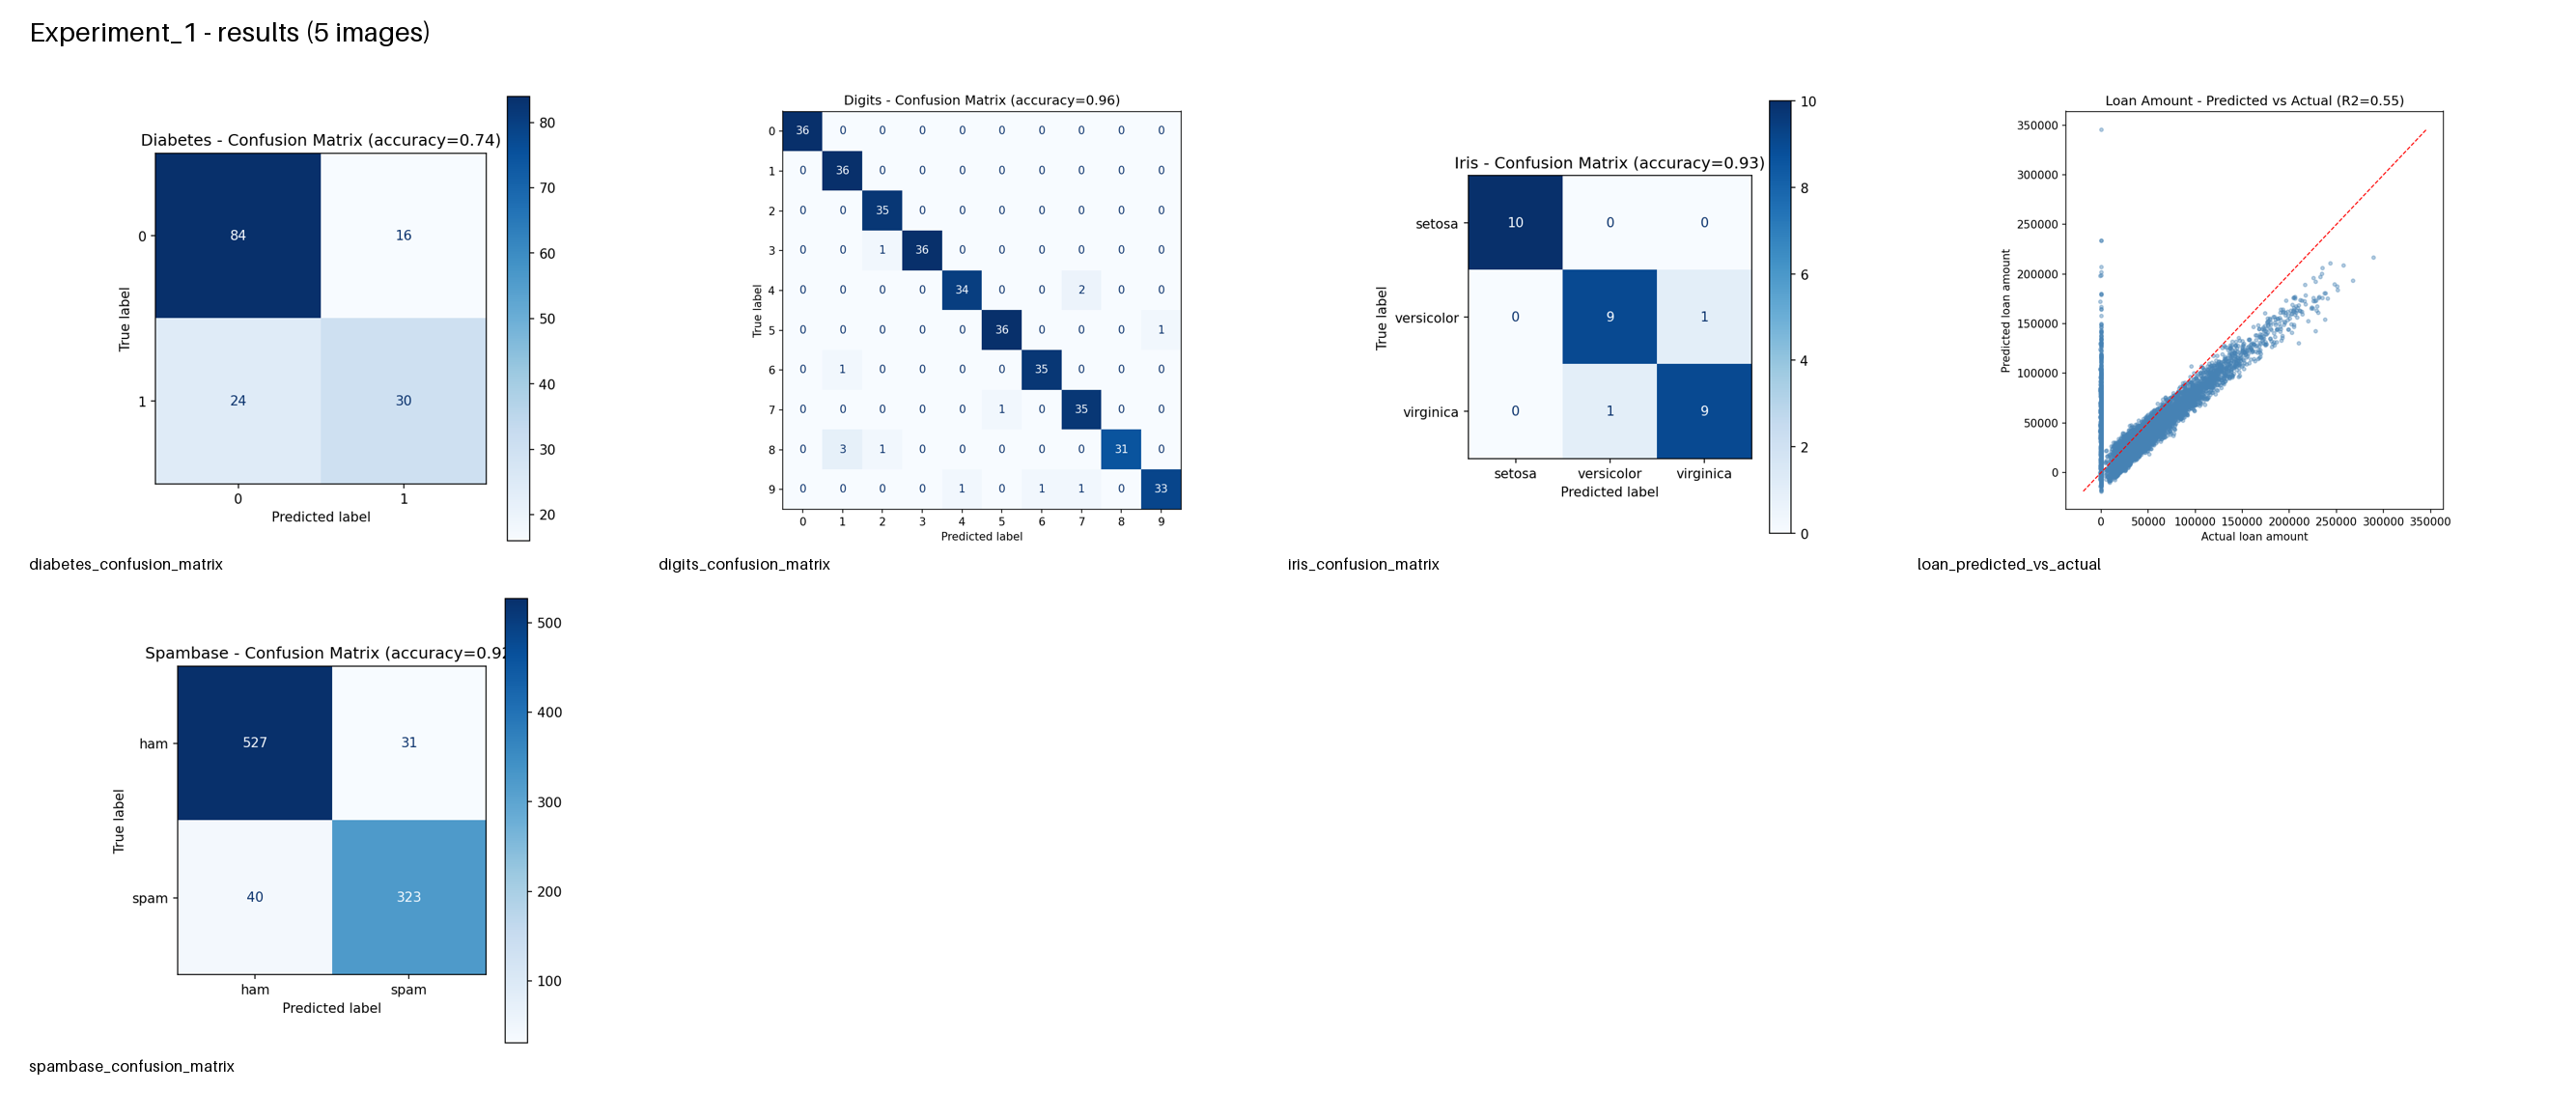
\includegraphics[width=0.9\linewidth]{outputs/Experiment_1_results_combined.png}
\caption{Confusion matrices for Iris, Diabetes, Spambase and Digits, and the predicted vs actual
scatter for the Loan Amount regression.}
\end{figure}

\textbf{Inference:}

Iris came out almost perfectly diagonal in its confusion matrix, just a couple of versicolor/virginica
mixups here and there, which is expected since those two species are known to blur together a bit. The
loan scatter plot tracks the diagonal reasonably well for small and medium loan amounts but starts
drifting for the biggest ones, makes sense, there just are not many huge loans in the data to learn
from. Diabetes leaned toward more false negatives than false positives, worth calling out since in a
medical context that is usually the more expensive kind of mistake to make. Spambase and Digits both
held up well, clean diagonals with only scattered errors.

\section{Discussion}
The workflow itself stayed consistent across every dataset, it was really only the specific technique
inside each step that had to change. None of the five baselines were tuned at all, so treat these
numbers as a floor rather than a ceiling on what each dataset can do. Diabetes came out the weakest of
the five, and that is probably down to a combination of a small sample (only 768 rows) and the known
quirk where several medical columns use 0 to mean "not recorded" instead of an actual zero.

\section{Conclusion}
The same six-step workflow held up cleanly across three different kinds of problems here, classification,
regression, and a multi-class image task. Iris and Digits gave the strongest baselines simply because
they are clean and well structured to begin with, while Loan Amount and Diabetes were tougher going,
mostly thanks to missing data and smaller, noisier feature sets.

\section{Learning Outcomes}
\begin{itemize}
\item Got real hands-on practice with the numpy, pandas, scipy, scikit-learn and matplotlib functions
that show up in basically every ML project.
\item Preprocessing needs change a lot depending on the dataset, clean data like Iris barely needs
anything while messy data like Loan Amount needs proper imputation and encoding work.
\item Learned to actually read a confusion matrix for what it is saying, not just glance at the
accuracy number and move on.
\item A baseline result with zero tuning is still worth having, it just tells you the floor you are
trying to beat later.
\end{itemize}

\section{References}
\begin{enumerate}
\item Stephen Marsland, ``Machine Learning - An Algorithmic Perspective'', 2nd Edition, Chapman and
Hall/CRC Machine Learning and Pattern Recognition Series, 2015.
\item Ethem Alpaydin, ``Introduction to Machine Learning'', 3rd Edition, The MIT Press, 2014.
\end{enumerate}

\end{document}
